Figure~\ref{fig:deconv} shows the
serial interval and incubation period distributions
from \cite{Du2020} and \cite{Lauer2020} respectively,
and the generation time distribution estimated via the proposed method.  %SM: figure 2 - in caption, indicate what S-hat refers to, and correct G to G-hat
The \mle parameters of $\hat{G}(\tau\mid\theta)$ were:
shape ${\alpha = 1.813}$ and scale ${\beta = 2.199}$,
yielding $\hat{S}(\tau\mid\theta^*)$ that closely approximated
the target $S(\tau)$.
\par
Comparison of the estimated generation time to serial interval distributions from the literature 
showed the following: the mean generation time of $3.99$ was similar to
the mean serial interval of $3.96$
based on the negative-permitting distribution \cite{Du2020},
but shorter than mean serial interval based on non-negative distributions,
such as $5.12$ in~\cite{Zhang2020} and $4.7$ in~\cite{Nishiura2020}.  %make it clear that using the same serial interval data for generation time and the fitted serial interval distributions [perhaps in methods?]
However, the \sd of the generation time distribution was smaller at $2.96$
than the \sd of the serial interval at $4.75$.   %non-negative fitted?  what about in comparison to the non-negative distributions?
Overall, estimated mean and \sd generation time
were similar to those reported by \textcite{Ganyani2020}  %SM: think the comparison is better suited for the discussion. i.e. comparison of the study results with existing literature.
(Table~\ref{tab:distr}).
\par
\begin{figure}
  \centering
  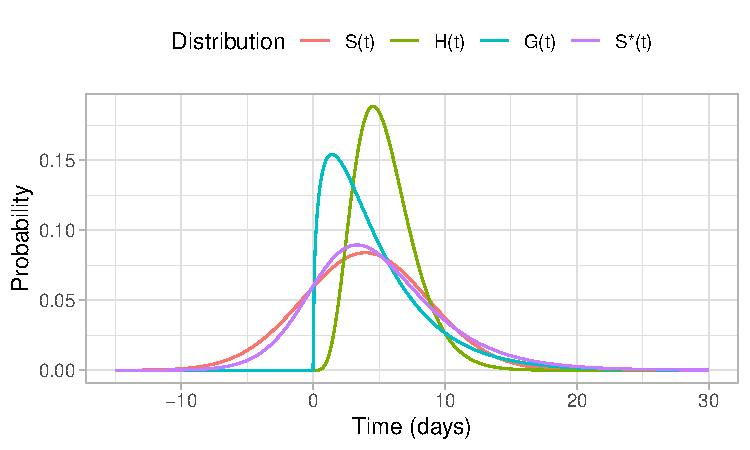
\includegraphics[width=\linewidth]{deconv}
  \caption{Recovery of the generation time distribution $G(\tau)$
    from the serial interval $S(\tau)$
    and incubation period $H(\tau)$ distributions}
  \label{fig:deconv}
\end{figure}
\par
Figure~\ref{fig:Re(t)} shows  %SM: can we zoom-in to the later dates? to show the differences more clearly after April 10 for example?
$\Re(t)$ for \covid in \gta, Canada
based on reported cases and estimated using
the generation time distribution versus
selected serial interval distributions reported in the literature.%
\footnote{Generation time and serial interval distributions
  are also illustrated in Figure~\ref{fig:distr-refs}.}
The $\Re(t)$ using the estimated generation time distribution
was lower (%SM - values using an early date and a later date)
compared to $\Re(t)$ based on non-negative serial interval distributions (%SM - values using an early date and a later date).  
%SM: currently the reason for this is not discussed. Could put in discussion but I think would be good to explain the 'why' here. 
The $\Re(t)$ estimated using
a negative-permitting serial interval distribution was the smallest of all three approaches %%SM - values here) 
%SM: given reason/explain 'why' here. 
\par
\begin{figure}[h]
  \centering
  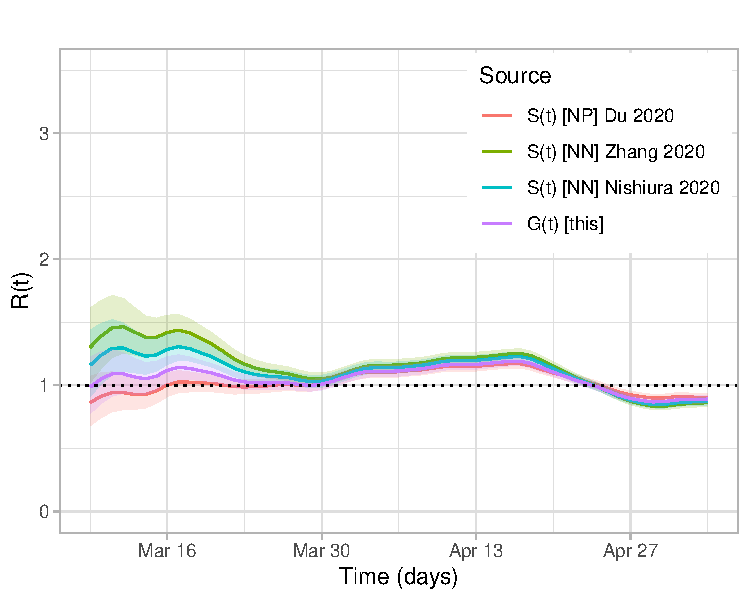
\includegraphics[width=\linewidth]{Re}
  \caption{$\Re(t)$ of \covid in \gta using
    serial interval versus generation time}
  \label{fig:Re(t)}
  \floatfoot{Notation ---
    $S(\tau)$:~serial interval;
    $G(\tau)$:~generation time;
    [NP]:~negative-permitting;
    [NN]:~non-negative.
  }
\end{figure}